\documentclass{article}
\usepackage{tikz}
\usetikzlibrary{shapes.multipart, positioning, arrows.meta}

\begin{document}
\begin{figure}[htbp]
\centering
\vspace{1cm}
\resizebox{\textwidth}{!}{
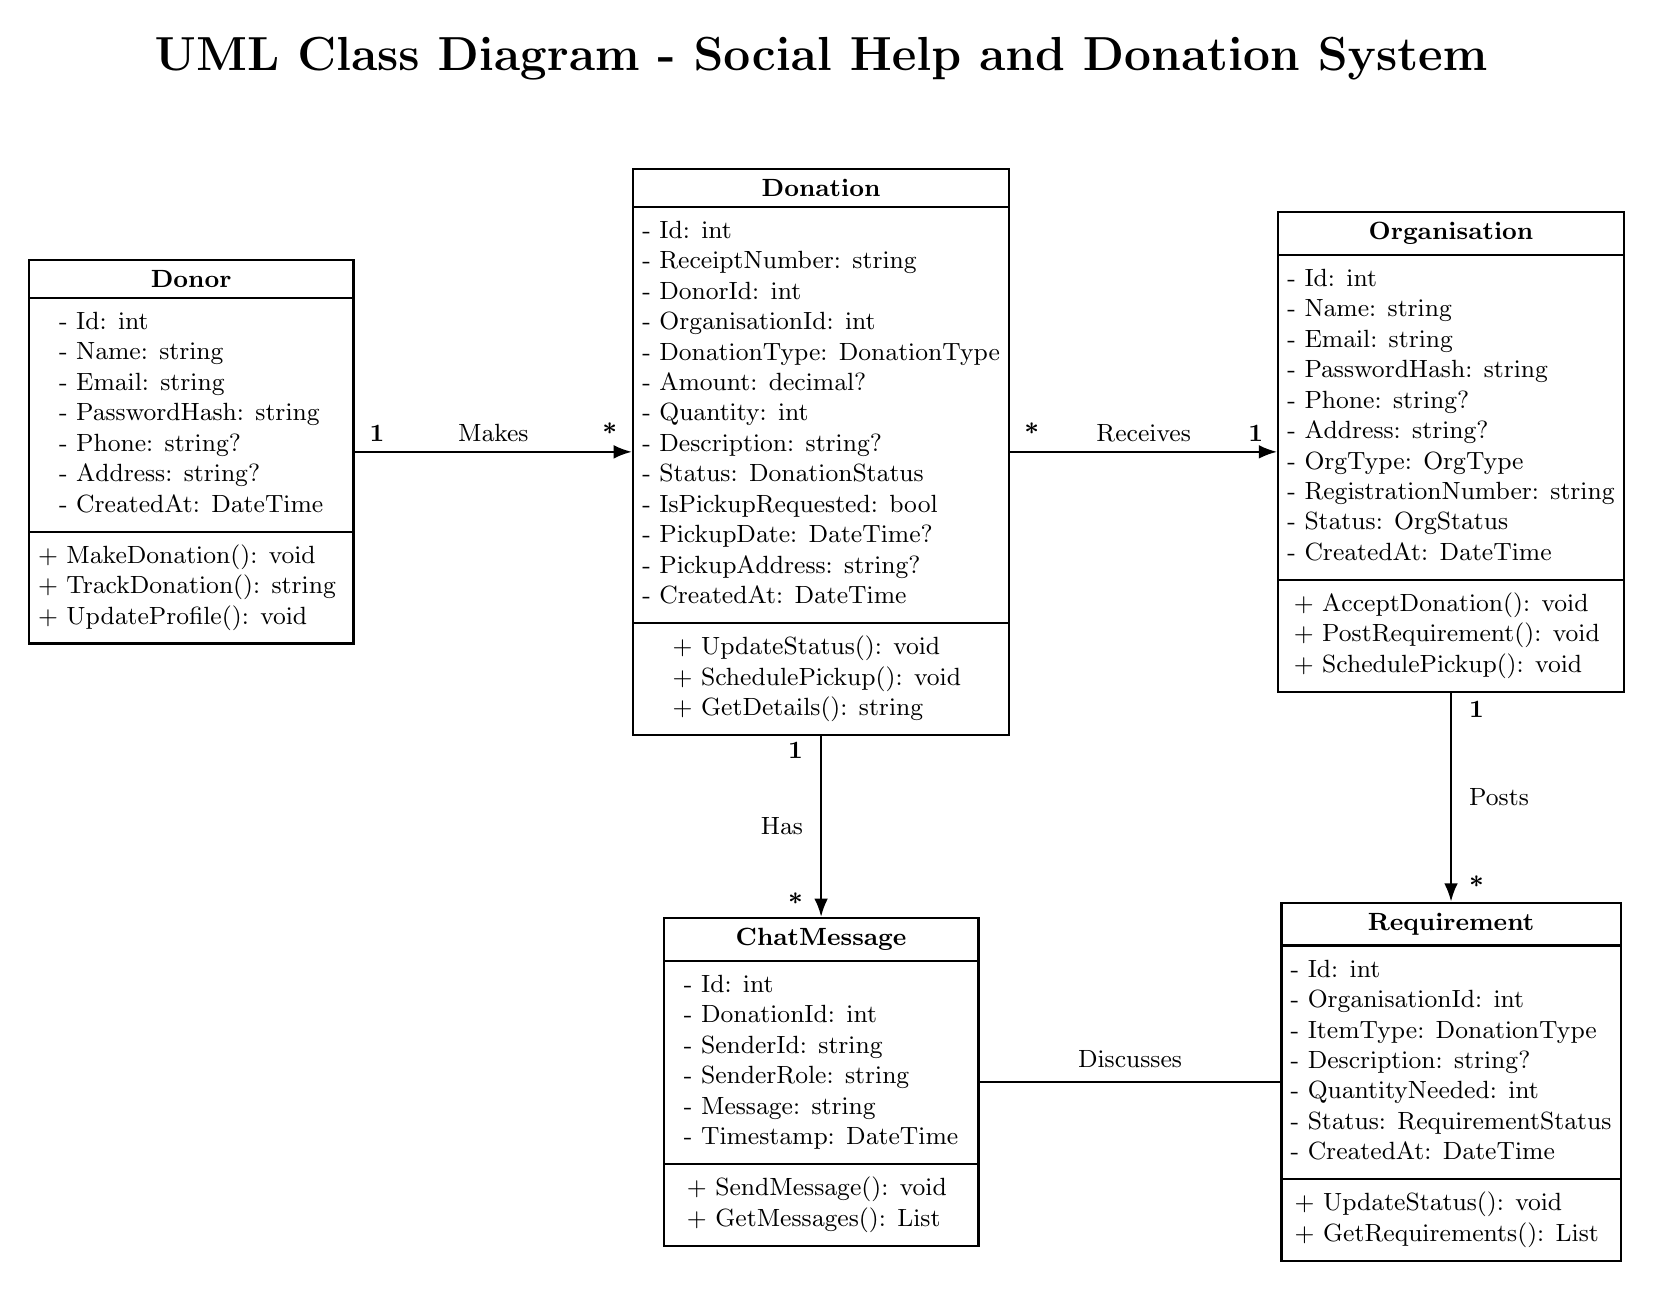
\begin{tikzpicture}[
    >=Latex,
    class/.style={
        draw, rectangle split, rectangle split parts=3,
        minimum width=4cm, align=center, fill=white, thick, font=\small
    }
]

% Title
\node[font=\LARGE\bfseries, align=center] at (0, 5) {UML Class Diagram - Social Help and Donation System};

% -------------------------
% Class Nodes Definition
% -------------------------

% 1. Donation (Center)
\node[class] (Donation) at (0, 0) {
    \textbf{Donation}
    \nodepart{second}
    \normalfont
    \begin{tabular}{@{}l@{}}
    - Id: int \\
    - ReceiptNumber: string \\
    - DonorId: int \\
    - OrganisationId: int \\
    - DonationType: DonationType \\
    - Amount: decimal? \\
    - Quantity: int \\
    - Description: string? \\
    - Status: DonationStatus \\
    - IsPickupRequested: bool \\
    - PickupDate: DateTime? \\
    - PickupAddress: string? \\
    - CreatedAt: DateTime
    \end{tabular}
    \nodepart{third}
    \normalfont
    \begin{tabular}{@{}l@{}}
    + UpdateStatus(): void \\
    + SchedulePickup(): void \\
    + GetDetails(): string
    \end{tabular}
};

% 2. Donor (Left)
\node[class] (Donor) at (-8, 0) {
    \textbf{Donor}
    \nodepart{second}
    \normalfont
    \begin{tabular}{@{}l@{}}
    - Id: int \\
    - Name: string \\
    - Email: string \\
    - PasswordHash: string \\
    - Phone: string? \\
    - Address: string? \\
    - CreatedAt: DateTime
    \end{tabular}
    \nodepart{third}
    \normalfont
    \begin{tabular}{@{}l@{}}
    + MakeDonation(): void \\
    + TrackDonation(): string \\
    + UpdateProfile(): void
    \end{tabular}
};

% 3. Organisation (Right)
\node[class] (Organisation) at (8, 0) {
    \textbf{Organisation}
    \nodepart{second}
    \normalfont
    \begin{tabular}{@{}l@{}}
    - Id: int \\
    - Name: string \\
    - Email: string \\
    - PasswordHash: string \\
    - Phone: string? \\
    - Address: string? \\
    - OrgType: OrgType \\
    - RegistrationNumber: string \\
    - Status: OrgStatus \\
    - CreatedAt: DateTime
    \end{tabular}
    \nodepart{third}
    \normalfont
    \begin{tabular}{@{}l@{}}
    + AcceptDonation(): void \\
    + PostRequirement(): void \\
    + SchedulePickup(): void
    \end{tabular}
};

% 4. Requirement (Bottom Right)
\node[class] (Requirement) at (8, -8) {
    \textbf{Requirement}
    \nodepart{second}
    \normalfont
    \begin{tabular}{@{}l@{}}
    - Id: int \\
    - OrganisationId: int \\
    - ItemType: DonationType \\
    - Description: string? \\
    - QuantityNeeded: int \\
    - Status: RequirementStatus \\
    - CreatedAt: DateTime
    \end{tabular}
    \nodepart{third}
    \normalfont
    \begin{tabular}{@{}l@{}}
    + UpdateStatus(): void \\
    + GetRequirements(): List
    \end{tabular}
};

% 5. ChatMessage (Bottom Center)
\node[class] (ChatMessage) at (0, -8) {
    \textbf{ChatMessage}
    \nodepart{second}
    \normalfont
    \begin{tabular}{@{}l@{}}
    - Id: int \\
    - DonationId: int \\
    - SenderId: string \\
    - SenderRole: string \\
    - Message: string \\
    - Timestamp: DateTime
    \end{tabular}
    \nodepart{third}
    \normalfont
    \begin{tabular}{@{}l@{}}
    + SendMessage(): void \\
    + GetMessages(): List
    \end{tabular}
};

% -------------------------
% Path Connections & Multiplicities
% -------------------------

% Donor -> Donation (1 to *)
\draw[->, thick] (Donor.east) -- (Donation.west)
    node[pos=0.08, above, font=\small\bfseries] {1}
    node[midway, above, font=\small] {Makes}
    node[pos=0.92, above, font=\small\bfseries] {*};

% Donation -> Organisation (* to 1)
\draw[->, thick] (Donation.east) -- (Organisation.west)
    node[pos=0.08, above, font=\small\bfseries] {*}
    node[midway, above, font=\small] {Receives}
    node[pos=0.92, above, font=\small\bfseries] {1};

% Donation -> ChatMessage (1 to *)
\draw[->, thick] (Donation.south) -- (ChatMessage.north)
    node[pos=0.08, left=0.1cm, font=\small\bfseries] {1}
    node[midway, left=0.1cm, font=\small] {Has}
    node[pos=0.92, left=0.1cm, font=\small\bfseries] {*};

% Organisation -> Requirement (1 to *)
\draw[->, thick] (Organisation.south) -- (Requirement.north)
    node[pos=0.08, right=0.1cm, font=\small\bfseries] {1}
    node[midway, right=0.1cm, font=\small] {Posts}
    node[pos=0.92, right=0.1cm, font=\small\bfseries] {*};

% ChatMessage -> Requirement (linking via Organisation context)
\draw[-, thick] (ChatMessage.east) -- (Requirement.west)
    node[midway, above=0.05cm, font=\small] {Discusses};

\end{tikzpicture}
}
\caption{UML Class Diagram for Social Help and Donation System}
\end{figure}
\end{document}
